\underbar{\textbf{\large Ejercicio 2:}} Sea el siguiente diagrama:
\begin{center}
  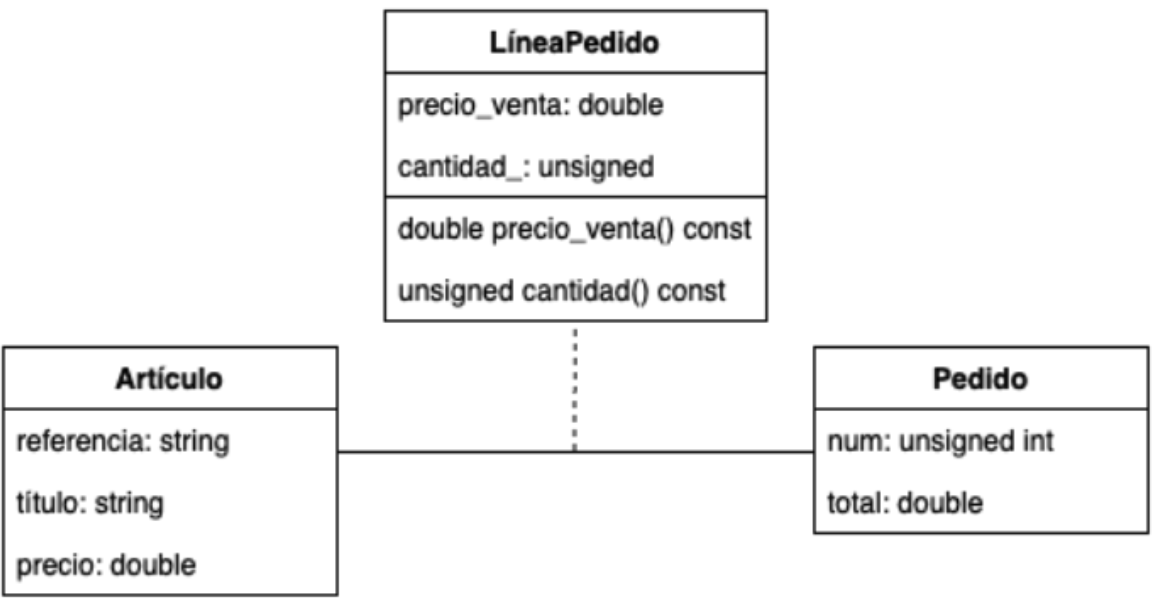
\includegraphics[width=0.7\textwidth]{assets/Febrero2023_1.png}
\end{center}
\begin{enumerate}[label = \alph*)]
  \item Defina la clase de asociación que permita implementar dicha relación escribiendo exclusivamente las definiciones de los miembros imprescindibles para implementarla.
  
  Como no tenemos una multiplicidad definida suponemos que es (N - 1..M).
\begin{minted}[breaklines]{C++}
class LineaPedido{};
class Articulo{}; //lado 1..M
class Pedido{}; //lado N

//Clase de asociación
class ArticuloPedido{
  public: 
    //Alias de las relaciones Articulo - LineaPedido y Pedido-LineaPedido
    typedef std::map<Articulo*,LineaPedido*>Articulos;
    typedef std::map<Pedido*,LineaPedido*>Pedidos;
    //Alias de las relaciones Articulo - Pedido
    typedef std::map<Articulo*,Pedidos>ArticulosPedidos;
    typedef std::map<Pedido*,Articulos>PedidosArticulos;

    void setArticuloPedido(Articulo& a, Pedido& p ,LineaPedido& lp)noexcept{
      directa[&a].insert(std::make_pair(&p,&lp));
      inversa[&p].insert(std::make_pair(&a,&lp));
    }
    void setArticuloPedido(Pedido& p, Articulo& a, LineaPedido& lp)noexcept{
      //Delegamos en la anterior
      setArticuloPedido(a,p,lp);
    }

    Articulos getArticulos(Pedido& p)const noexcept{
      auto i = inversa.find(&p);
      if(i!=inversa.end())return i->second;
      return std::map<Articulo*,LineaPedido*>();
    }
    const Pedidos& getPedidos(Articulo& a)const noexcept{
      return directa.find(&a)->second;
    }

  private:    
    ArticulosPedidos directa;
    PedidosArticulos inversa;
};
\end{minted}
  \item ¿Es obligatorio usar una clase de asociación? Si es así explica razonadamente el porqué, si no, implementa como hacerlo escribiendo las declaraciones de los miembros esenciales.
  
  No, no es obligatorio, las relaciones de asociación podemos implementarla de dos maneras, haciendo la clase de asociación ó incluyendo los miembros imprescindibles en cada clase para que la relación se pueda llevar a cabo.
\begin{minted}[breaklines]{C++}
class Articulo{
  public:
    //Métodos propios de la clase
    //Alias del diccionario que recibe de la relacion con Pedido
    typedef std::map<Pedido*,LineaPedido*>Pedidos;
    void setPedido(Pedido& p,LineaPedido& lp)noexcept{
      pedidos_.insert(std::make_pair(&p,&lp));
    }
    const Pedidos& getPedidos()const noexcept{return pedidos_;}
  private:
    //Atributos propios de la clase
    Pedidos pedidos_; //nombre del diccionario.
};

class Pedido{
  public:
    //Método propios de la clase
    //Alias del diccionario que recibe de la relación con Articulo.
    typedef std::map<Articulo*,LineaPedido*>Articulos;
    Pedido(Articulo& a, LineaPedido& lp,/*Atributos de la clase*/) {
      setArticulo(a,lp);
    }
    void setArticulo(Articulo& a,LineaPedido& lp)noexcept{
      articulos_.insert(std::make_pair(&a,&lp));
    }
    const Articulos& getArticulo()const noexcept{return articulos_;}
  private:
    //Atributos propios de la clase
    Articulos articulos_;
};
\end{minted}
\end{enumerate}
\newpage
\underbar{\textbf{\large Ejercicio 3:}} Sea la clase ListaOrdenada:
\begin{center}
  \begin{lstlisting}[frame = single]
template<typename T>
class ListaOrdenada{
  public:
      typedef typename list<T>::const_iterator iterator;
      void insertar(const T& e);
      void eliminar(iterator p);

      iterator begin();
      iterator end();
};
  \end{lstlisting}
\end{center}
\begin{enumerate}[label = \alph*)]
  \item Explica la relación que se puede establecer entre ListaOrdenada y la clase list. Implemente la clase ListaOrdenada.
  
  Una ListaOrdenada podemos pensarlo como un tipo de lista donde sus elementos están ordenados mediante un criterio de ordenación a diferencia de list que será una lista con sus elementos desordenados.
  Por tanto, como no tienen el mismo comportamiento no podemos hacer que list se especialice en una ListaOrdenada pero si podemos delegar parte del comportamiento de list en la clase ListaOrdenada. Por ello, vamos a implementarla mediante una relación de composición 1 - 1 que se puede hacer mediante herencia privada o inclusión de un Objeto list.
\begin{minted}[breaklines]{C++}
  template<typename T>
  class ListaOrdenada{
    public:
        typedef typename list<T>::const_iterator iterator;
        ListaOrdenada():list<T>(){}
        void insertar(const T& e);
        void eliminar(iterator p);
  
        iterator begin();
        iterator end();
    private:
      list<T>listaordenada_; //objeto de tipo list
  };
\end{minted}
\newpage
  \item Añade el método \texttt{size\_t contar (const T\& e)} const que cuente el número de ocurrencias de un elemento dado. Para ello utilice \texttt{count\_if()} de la clase STL que recibe dos iteradores y un predicado (clase objeto función que devuelve un booleano). Defina el predicado como una clase de objetos función o como una función anónima (función lambda) equivalente.
\end{enumerate}
\begin{minted}[breaklines]{C++}
template<typename T>
class ListaOrdenada{
  public:
      typedef typename list<T>::const_iterator iterator;
      ListaOrdenada():list<T>(){}
      void insertar(const T& e){
        //Como vamos a insertar ordenadamante, haremos uso de lower_bound, que nos devuelve un iterador al primer elemento menor que el.
        auto p = std::lower_bound(listaordenada_.begin(),listaordenada_.end(),e);
        //insertamos el elemento
        listaordenada_.insert(p,e);
      }
      void eliminar(iterator p){
        listaordenada_.erase(p);

      }
      size_t contar(const T& e)const{
        //Para contar nos dice que hagamos uso de count_if
        return count_if(listaordenada_.begin(),listaordenada_.end(),[&e](const T& elto){return elto == e ;});
      }
      iterator begin(){return listaordenada_.cbegin();}
      iterator end(){return listaordenada_.cend();}
  private:
    list<T>listaordenada_; //composición
};
\end{minted}
\newpage
\underbar{\textbf{\large Ejercicio 4:}} Sea el siguiente código:
\begin{center}
  \begin{lstlisting}[frame = single]
class Instrumento{
  public:
    typedef enum {instrumento, percusion, cuerda, viento}tClase;
    Instrumento(string nom):nombre_(nom){clase_ = instrumento;}

    void tocar()const{
      cout<<"Soy un "<<nombre()<<" y pertenezco a "<<clase()<<endl;
    }

    string nombre() const{return nombre_;}
    string clase()const{
      switch (clase_){
      case percusion: return "percusion";
      case cuerda: return "cuerda";
      case viento: return "viento";
      default: return "instrumento";
      }
    }
  protected:
    string nombre_;
    tClase clase_;
};

class Percusion:public Instrumento{
    Percusion(string n):Instrumento(n){clase_ = percusion;}
};  

class Cuerda: public Instrumento{
    Cuerda(string n):Instrumento(n){clase_ = cuerda;}
};

class Viento: public Instrumento{
    Viento(string n):Instrumento(n){clase_=viento;}
};
  \end{lstlisting}
\end{center}

\begin{enumerate}[label = \alph*)]
  \item ¿Se puede mejorar la implementación de esta jerarquía de clases usando métodos polimórficos? En caso afirmativo, reescribe el programa para obtener un resultado idéntico.
  
  Si, como vemos no estamos haciendo uso de polimorfísmo en ningún momento, simplmente estamos creando objetos de tipo Instrumento y asignándoles una clase en particular.
  Si hacemos uso de polimorfísmo tanto ese método clase() como el enum desaparecerían ya que la clase se asignaría en cada constructor de las clases Derivadas de Instrumento, además que cada clase derivada tendría su propio método tocar(), quedando:
\begin{minted}[breaklines]{C++}
class Instrumento{
  public:
    Instrumento(string nom):nombre_(nom){}
    virtual void tocar()const{
      cout<<"Soy un "<<nombre()<<" y pertenezco a Instrumento"<<endl;
    }
    string nombre() const{return nombre_;}
    virtual ~Instrumento() =default; //Es polimorfica, destructor virtual.
  protected:
    string nombre_;
};

class Percusion:public Instrumento{
  public:
    Percusion(string n):Instrumento(n){}
    void tocar()const override {
      cout<<"Soy un "<<nombre()<<" y pertenezco a Tambor"<<endl;
    }
    string nombre()const {return nombre_;}
};  

class Cuerda: public Instrumento{
  public:
    Cuerda(string n):Instrumento(n){}
     void tocar()const override{
      cout<<"Soy un "<<nombre()<<" y pertenezco a Cuerda"<<endl;
    }
    string nombre()const {return nombre_;}
};

class Viento: public Instrumento{
  public:
    Viento(string n):Instrumento(n){}
    void tocar()const override{
      cout<<"Soy un "<<nombre()<<" y pertenezco a Viento"<<endl;
    }
    string nombre()const {return nombre_;}
};
\end{minted}
  \item Implemente una función que clasifique un vector de punteros a instrumentos en otros 3 vectores de punteros a instrumentos, uno para cada clase: percusión, cuerda y viento, ignorando aquellos que no pertenezcan a estas clases.
\begin{minted}[breaklines]{C++}
void clasificaInstrumento(vector<Instrumento*>&instrumentos, vector<Percusion*>& percusiones, vector<Viento*>& vientos, vector<Cuerda*>& cuerdas){
  //convertimos los instrumentos en su tipo, y los guardamos en sus vectores
  for(auto i : instrumentos)
    if(Percusion* pp = dynamic_cast<Percusion*>(i)){ percusiones.push_back(pp);
    }
    else if(Viento* pv = dynamic_cast<Viento*>(i)){ vientos.push_back(pv);
    }
    else if(Cuerda* pc= dynamic_cast<Cuerda*>(i)){ cuerdas.push_back(pc);
    }
}
\end{minted}
\end{enumerate}
